\حصہء{سوالات}
\موٹا{حد کی تلاش}\\
سوال \حوالہ{سوال_ترتیب_مرتکز_منفرج_الف} تا سوال \حوالہ{سوال_ترتیب_مرتکز_منفرج_ب} میں کون سی ترتیب \عددی{\{a_n\}}  مرتکز اور کون سی منفرج ہے؟ ہر مرتکز ترتیب کا حد تلاش کریں۔

\ابتدا{سوال}\شناخت{سوال_ترتیب_مرتکز_منفرج_الف}
$a_n=2+(0.1)^n$
\انتہا{سوال}
%=====================
\ابتدا{سوال}
$a_n=\frac{n+(-1)^n}{n}$
\انتہا{سوال}
%====================
\ابتدا{سوال}
$a_n=\frac{1-2n}{1+2n}$
\انتہا{سوال}
%====================
\ابتدا{سوال}
$a_n=\frac{2n+1}{1-3\sqrt{n}}$
\انتہا{سوال}
%====================
\ابتدا{سوال}
$a_n=\frac{1-5n^4}{n^4+8n^3}$
\انتہا{سوال}
%====================
\ابتدا{سوال}
$a_n=\frac{n+3}{n62+5n+6}$
\انتہا{سوال}
%====================
\ابتدا{سوال}
$a_n=\frac{n62-2n+1}{n-1}$
\انتہا{سوال}
%====================
\ابتدا{سوال}
$a_n=\frac{1-n^3}{70-4n^2}$
\انتہا{سوال}
%====================
\ابتدا{سوال}
$a_n=1+(-1)^n$
\انتہا{سوال}
%====================
\ابتدا{سوال}
$a_n=(-1)^n(1-\tfrac{1}{n})$
\انتہا{سوال}
%====================
\ابتدا{سوال}
$a_n=(\tfrac{n+2}{2n})(1-\tfrac{1}{n})$
\انتہا{سوال}
%====================
\ابتدا{سوال}
$a_n=(2-\tfrac{1}{2^n})(3+\tfrac{1}{2^n})$
\انتہا{سوال}
%====================
\ابتدا{سوال}
$a_n=\frac{(-1)^{n+1}}{2n-1}$
\انتہا{سوال}
%====================
\ابتدا{سوال}
$a_n=(-\tfrac{1}{2})^n$
\انتہا{سوال}
%====================
\ابتدا{سوال}
$a_n=\sqrt{\frac{2n}{n+1}}$
\انتہا{سوال}
%====================
\ابتدا{سوال}
$a_n=\frac{1}{(0.9)^n}$
\انتہا{سوال}
%====================
\ابتدا{سوال}
$a_n=\sin(\tfrac{\pi}{2}+\tfrac{1}{n})$
\انتہا{سوال}
%====================
\ابتدا{سوال}
$a_n=n\pi \cos (n\pi)$
\انتہا{سوال}
%====================
\ابتدا{سوال}
$a_n=\frac{\sin n}{n}$
\انتہا{سوال}
%====================
\ابتدا{سوال}
$a_n=\frac{\sin^2 n}{2^n}$
\انتہا{سوال}
%====================
\ابتدا{سوال}
$a_n=\frac{n}{2^n}$
\انتہا{سوال}
%====================
\ابتدا{سوال}
$a_n=\frac{3^n}{n^3}$
\انتہا{سوال}
%====================
\ابتدا{سوال}
$a_n=\frac{\ln(n+1)}{\sqrt{n}}$
\انتہا{سوال}
%====================
\ابتدا{سوال}
$a_n=\frac{\ln n}{\ln 2n}$
\انتہا{سوال}
%====================
\ابتدا{سوال}
$a_n=8^{1/n}$
\انتہا{سوال}
%====================
\ابتدا{سوال}
$a_n=(0.03)^{1/n}$
\انتہا{سوال}
%====================
\ابتدا{سوال}
$a_n=(1+\tfrac{7}{n})^n$
\انتہا{سوال}
%====================
\ابتدا{سوال}
$a_n=(1-\tfrac{1}{n})^n$
\انتہا{سوال}
%====================
\ابتدا{سوال}
$a_n=\sqrt[n]{10n}$
\انتہا{سوال}
%====================
\ابتدا{سوال}
$a_n=\sqrt[n]{n^2}$
\انتہا{سوال}
%====================
\ابتدا{سوال}
$a_n=(\tfrac{3}{n})^{1/n}$
\انتہا{سوال}
%====================
\ابتدا{سوال}
$a_n=(n+4)^{1/(n+4)}$
\انتہا{سوال}
%====================
\ابتدا{سوال}
$a_n=\frac{\ln n}{n^{1/n}}$
\انتہا{سوال}
%====================
\ابتدا{سوال}
$a_n=\ln n-\ln(n+1)$
\انتہا{سوال}
%====================
\ابتدا{سوال}
$a_n=\sqrt[n]{4^nn}$
\انتہا{سوال}
%====================
\ابتدا{سوال}
$a_n=\sqrt[n]{3^{2n+1}}$
\انتہا{سوال}
%====================
\ابتدا{سوال}
$a_n=\frac{n!}{n^n}$\quad
(اشارہ: \عددی{\tfrac{1}{n}} کے ساتھ موازنہ کریں) 
\انتہا{سوال}
%====================
\ابتدا{سوال}
$a_n=\frac{(-4)^n}{n!}$
\انتہا{سوال}
%====================
\ابتدا{سوال}
$a_n=\frac{n!}{10^{6n}}$
\انتہا{سوال}
%====================
\ابتدا{سوال}
$a_n=\frac{n!}{2^n\cdot 3^n}$
\انتہا{سوال}
%====================
\ابتدا{سوال}
$a_n=(\tfrac{1}{n})^{1/(\ln n)}$
\انتہا{سوال}
%====================
\ابتدا{سوال}
$a_n=\ln(1+\tfrac{1}{n})^n$
\انتہا{سوال}
%====================
\ابتدا{سوال}
$a_n=(\tfrac{3n+1}{3n-1})^n$
\انتہا{سوال}
%====================
\ابتدا{سوال}
$a_n=(\tfrac{n}{n+1})^n$
\انتہا{سوال}
%====================
\ابتدا{سوال}
$a_n=(\tfrac{x^n}{2n+1})^{1/n},\quad x>0$
\انتہا{سوال}
%====================
\ابتدا{سوال}
$a_n=(1-\tfrac{1}{n^2})^n$
\انتہا{سوال}
%====================
\ابتدا{سوال}
$a_n=\frac{3^n\cdot 6^n}{2^{-n}\cdot n!}$
\انتہا{سوال}
%====================
\ابتدا{سوال}
$a_n=\frac{(10/{11})^n}{(9/{10})^n+(11/{12})^n}$
\انتہا{سوال}
%====================
\ابتدا{سوال}
$a_n=\tanh n$
\انتہا{سوال}
%====================
\ابتدا{سوال}
$a_n=\sinh (\ln n)$
\انتہا{سوال}
%====================
\ابتدا{سوال}
$a_n=\frac{n^2}{2n-1}\sin\frac{1}{n}$
\انتہا{سوال}
%====================
\ابتدا{سوال}
$a_n=n(1-\cos\frac{1}{n})$
\انتہا{سوال}
%====================
\ابتدا{سوال}
$a_n=\tan^{-1}n$
\انتہا{سوال}
%====================
\ابتدا{سوال}
$a_n=\frac{1}{\sqrt{n}}\tan^{-1}n$
\انتہا{سوال}
%====================
\ابتدا{سوال}
$a_n=(\tfrac{1}{3})^n+\frac{1}{\sqrt{2^n}}$
\انتہا{سوال}
%====================
\ابتدا{سوال}
$a_n=\sqrt[n]{n^2+n}$
\انتہا{سوال}
%====================
\ابتدا{سوال}
$a_n=\frac{(\ln n)^{200}}{n}$
\انتہا{سوال}
%====================
\ابتدا{سوال}
$a_n=\frac{(\ln n)^5}{\sqrt{n}}$
\انتہا{سوال}
%====================
\ابتدا{سوال}
$a_n=n-\sqrt{n^2-n}$
\انتہا{سوال}
%====================
\ابتدا{سوال}
$a_n=\frac{1}{\sqrt{n^2-1}-\sqrt{n^2+n}}$
\انتہا{سوال}
%====================
\ابتدا{سوال}
$a_n=\frac{1}{n}\int_1^n \frac{\dif x}{x}$
\انتہا{سوال}
%====================
\ابتدا{سوال}\شناخت{سوال_ترتیب_مرتکز_منفرج_ب}
$a_n=\int_1^n\frac{\dif x}{x^p},\quad p>1$
\انتہا{سوال}
%====================
\موٹا{نظریہ اور مثالیں}\\
\ابتدا{سوال}
ایک ترتیب کی پہلی جزو  \عددی{x_1=1} ہے۔ ہر اگلا جزو گزشتہ تمام اجزاء کا مجموعہ ہے:
\begin{align*}
x_{n+1}=x_1+x_2+\cdots+x_{n}
\end{align*}
ابتدائی چند اجزاء لکھ کر عمومی جزو \عددی{x_n} کا کلیہ \عددی{n\ge 2} کے لئے تلاش کریں۔ 
\انتہا{سوال}
%====================
\ابتدا{سوال}
ناطق اعداد کی درج ذیل ترتیب میں نسب نما ایک ترتیب، شمار کنندہ دوسری ترتیب اور ان کی نسبت تیسری ترتیب ہے۔
\begin{align*}
\frac{1}{2},\frac{3}{2},\frac{7}{5},\frac{17}{12},\cdots,\frac{a}{b},\frac{a+2b}{a+b}
\end{align*} 
\عددی{x_n} اور \عددی{y_n} کو بالترتیب \عددی{n} ویں نسبت \عددی{r_n=\tfrac{x_n}{y_n}} کا نسب نما اور شمار کنندہ تصور کریں۔
\begin{enumerate}[a.]
\item
\عددی{x_1^2-2y_1^2=-1} اور \عددی{x_2^2-2y_2^2=+1} کی تصدیق کریں۔ ساتھ ہی \عددی{a^2-2b^2=\mp1}  کی صورت  میں  \عددی{(a+2b)^2-2(a+b)^2=\pm1}  کی تصدیق کریں۔
\item
\عددی{n} بڑھانے سے کسر \عددی{r_n=\tfrac{x_n}{y_n}} ایک حد تک پہنچتا ہے۔ یہ حد کیا ہے؟ (اشارہ: جزو-ا استعمال کرتے ہوئے \عددی{r_n^2-2=\pm(\tfrac{1}{y_n})^2} دکھائیں اور دکھائیں کہ \عددی{y_n\ge n} ہے۔)
\end{enumerate}
\انتہا{سوال}
%====================
\ابتدا{سوال}\موٹا{ترکیب نیوٹن}\\
ترکیب نیوٹن درج ذیل کلیہ توالی دیتا ہے۔
\begin{align*}
x_{n+1}=x_n-\frac{f(x_n)}{f'(x_n)}
\end{align*}
کیا یہ ترتیب مرتکز ہے؟ اگر مرتکز ہے تب کس حد کو مرتکز ہے؟  تفاعل \عددی{f} پہچانیں جو درج ذیل ترتیب دیتا ہے۔
\begin{align*}
\text{\RL{(الف)}}&&x_0&=1,&&x_{n+1}=x_n-\frac{x_n^2-2}{2x_n}=\frac{x_n}{2}+\frac{1}{x_n}\\
\text{\RL{(ب)}}&&x_0&=1,&&x_{n+1}=x_n-\frac{\tan x_n-1}{\sec^2x_n}\\
\text{\RL{(ج)}}&&x_0&=1,&&x_{n+1}=x_n-1
\end{align*}
\انتہا{سوال}
%========================
\ابتدا{سوال}
(الف) فرض کریں وقفہ \عددی{[0,1]} میں تمام \عددی{x} پر \عددی{f(x)} قابل تفرق ہے اور \عددی{f(0)=0} ہے۔ ترتیب \عددی{\{a_n\}} کو \عددی{a_n=nf(\tfrac{1}{n})} پیش کرتی ہے۔ دکھائیں کہ \عددی{\lim_{n\to\infty}a_n=f'(0)} ہو گا۔

جزو-الف کا نتیجہ استعمال کرتے ہوئے جزو-ب تا جزو د میں دیے ترتیبات کے حد تلاش کریں۔ (ب) \عددی{a_n=n\tan^{-1}\tfrac{1}{n}}، (ج) \عددی{a_n=n(e^{1/n}-1)}، (د) \عددی{a_n=n\ln (1+\tfrac{2}{n})}
\انتہا{سوال}
%====================
\ابتدا{سوال}\شناخت{سوال_ترکیب_فیثاغورث_جوڑی}\ترچھا{تین کی فیثاغوری جوڑی}\\
اگر \عددی{a^2+b^2=c^2} ہو تب \عددی{a}، \عددی{b} اور \عددی{c} کو تین کی فیثاغوری جوڑی کہتے ہیں۔ فرض کریں \عددی{a} ایک طاق مثبت عدد صحیح  جبکہ
\begin{align*}
c=\lceil\tfrac{a^2}{2}\rceil\quad \text{اور}\quad b=\lfloor\tfrac{a^2}{2}\rfloor^2
\end{align*}
بالترتیب \عددی{\tfrac{a^2}{2}} کے عدد صحیح زمین اور عدد صحیح چھت تفاعل ہیں۔
\begin{enumerate}[a.]
\item
دکھائیں \عددی{a^2+b^2=c^2} (اشارہ:  \عددی{a=2n+1} لے کر \عددی{b} اور \عددی{c} کو \عددی{n} کی صورت میں لکھیں۔)
\item
بلا واسطہ حساب سے یا شکل \حوالہ{شکل_سوال_ترکیب_فیثاغورث_جوڑی} کی مدد سے \عددی{\lim_{a\to\infty}\tfrac{\lfloor a^2/2\rfloor}{\lceil a^2/2\rceil}} تلاش کریں۔
\end{enumerate}
\begin{figure}
\centering
\begin{tikzpicture}
\pgfmathsetmacro{\ang}{atan(1.5)}
\draw(0,0)--(1,0)node[pos=0.5,below]{$a$}--++(0,1.5)node[pos=0.5,right]{$\lfloor \tfrac{a^2}{2}\rfloor$}--(0,0)node[pos=0.4,left]{$\lceil \tfrac{a^2}{2}\rceil$};
\draw([shift={(0:0.3)}]0,0) arc (0:\ang:0.3);
\draw(\ang/2:0.5)node[]{$\theta$};
\end{tikzpicture}
\caption{فیثاغوری تین کی جوڑی (سوال \حوالہ{سوال_ترکیب_فیثاغورث_جوڑی})}
\label{شکل_سوال_ترکیب_فیثاغورث_جوڑی}
\end{figure}
\انتہا{سوال}
%=================
\ابتدا{سوال}\ترچھا{\عددی{n!} کا \عددی{n} واں جذر}\\
\begin{enumerate}[a.]
\item
دکھائیں کہ \عددی{\lim_{a\to\infty}(2n\pi)^{1/(2n)}=1} ہے اور  تخمین سٹرلنگ استعمال کرتے ہوئے دکھائیں کہ \عددی{n} کی بڑی قیمتوں کے لئے  \عددی{\sqrt[n]{n!}\approx \tfrac{n}{e}} ہو گا۔
\item
جہاں تک آپ کا کیلکولیٹر نتائج دے سکتا ہے وہاں تک \عددی{n=40,50,60,\cdots} کے لئے کیلکولیٹر سے حاصل \عددی{\sqrt[n]{n!}} کے نتائج کا جزو-الف کے کلیہ سے حاصل نتائج کے ساتھ موازنہ کریں۔ 
\end{enumerate}
\انتہا{سوال}
%==================
\ابتدا{سوال}
(ا) فرض کریں کسی بھی مثبت مستقل \عددی{c} کے لئے \عددی{\lim_{n\to\infty}(\tfrac{1}{n^c})=0} ہے۔ اب دکھائیں \عددی{\lim_{n\to\infty}\tfrac{\ln n}{n^c}=0} ہو گا۔ (ب) کسی بھی مثبت مستقل \عددی{c} کے لئے ثابت کریں کہ \عددی{\lim_{n\to\infty}(\tfrac{1}{n^c})=0} ہو گا۔ (اشارہ: اگر \عددی{\epsilon=0.001} اور \عددی{c=0.04} ہوں تب \عددی{n>N} کی صورت میں \عددی{\abs{\tfrac{1}{n^c}-0}<\epsilon} کے لئے \عددی{N} کتنا بڑا ہونا چاہیے؟)
\انتہا{سوال}
%===============
\ابتدا{سوال}
اگر \عددی{\{a_n\}} اور \عددی{\{b_n\}} دونوں \عددی{L} پر مرتکز ہوں تب دکھائیں کہ ترتیب \عددی{a_1,b_1,a_2,b_2,\cdots,a_n,b_n,\cdots} بھی \عددی{L} پر مرتکز ہو گی۔
\انتہا{سوال}
%=====================
\ابتدا{سوال}
ثابت کریں \عددی{\lim_{n\to\infty}\sqrt[n]{n}=1}
\انتہا{سوال}
%================
\ابتدا{سوال}
ثابت کریں \عددی{\lim_{n\to\infty}x^{1/n}=1} جہاں \عددی{x>0} ہے۔
\انتہا{سوال}
%======================
\ابتدا{سوال}
ثابت کریں مسئلہ \حوالہ{مسئلہ_ترتیب_قواعد_حد_ج}
\انتہا{سوال}
%=================
\ابتدا{سوال}
ثابت کریں مسئلہ \حوالہ{مسئلہ_ترتیب_قواعد_حد_د}
\انتہا{سوال}
%=================
\موٹا{ترکیب پکاغ}\\
سوال \حوالہ{سوال_ترکیب_ترکیب_پکاغ_الف} تا سوال \حوالہ{سوال_ترکیب_ترکیب_پکاغ_ب} میں دیے گئے مساوات کو ترکیب پکاغ سے حل کریں۔

\ابتدا{سوال}\شناخت{سوال_ترکیب_ترکیب_پکاغ_الف}
$\sqrt{x}=x$
\انتہا{سوال}
%======================
\ابتدا{سوال}
$x^2=x$
\انتہا{سوال}
%========================
\ابتدا{سوال}
$\cos x+x=0$
\انتہا{سوال}
%========================
\ابتدا{سوال}
$\cos x=x+1$
\انتہا{سوال}
%========================
\ابتدا{سوال}
$x-\sin x=0.1$
\انتہا{سوال}
%========================
\ابتدا{سوال}\شناخت{سوال_ترکیب_ترکیب_پکاغ_ب}
$\sqrt{x}=4-\sqrt{1+x}$\quad
(اشارہ: پہلے دونوں اطراف کا مربع لیں۔)
\انتہا{سوال}
%========================
\ابتدا{سوال}
ترکیب پکاغ سے \عددی{\sqrt{x}=x} کا حل \عددی{x=1} تلاش کریں جبکہ اس کے حل \عددی{x=0} اس ترکیب سے تلاش مت کریں۔ کیوں؟ (اشارہ: \عددی{y=x} اور \عددی{y=\sqrt{x}} کو ایک ساتھ ترسیم کریں۔)
\انتہا{سوال}
%========================
\ابتدا{سوال}
ترکیب پکاغ میں \عددی{\abs{x_0}\ne 1} لے کر \عددی{x^2=x} کا حل  \عددی{x=0} تلاش کیا جا سکتا ہے جبکہ اس کے حل \عددی{x=1} اس ترکیب سے تلاش نہیں کیا جا سکتا ہے۔ کیوں؟ (اشارہ: \عددی{y=x} اور \عددی{y=x^2} کو ایک ساتھ ترسیم کریں۔)
\انتہا{سوال}
%========================

\ترچھا{اکائی سے زیادہ ڈھلوان}\\
ہم نے مثال \حوالہ{مثال_ترتیب_پرکھ_پکاغ_سوم} میں دیکھا کہ \عددی{g(x)=4x-12} کے مقررہ نقطہ کو ترکیب پکاغ سے حاصل نہیں کیا جا سکتا ہے جبکہ  \عددی{g^{-1}(x)=\tfrac{1}{4}x+3} کا مقررہ نقطہ ترکیب پکاغ سے حاصل کیا جا سکتا ہے چونکہ کسی بھی وقفہ پر \عددی{g^{-1}} کے تفرق  کی مطلق مقدار \عددی{\tfrac{1}{4}} ہے جو \عددی{1} سے کم ہے۔ مثال \حوالہ{مثال_ترتیب_پرکھ_پکاغ} میں ہم نے دیکھا کہ \عددی{g^{-1}} کا مقررہ نقطہ \عددی{x=4} ہے  جو \عددی{g(4)=4(4)-12=4} کی بنا \عددی{g} کا بھی مقررہ نقطہ ہے۔ یوں \عددی{g^{-1}} کا مقررہ نقطہ تلاش کرتے ہوئے ہم نے \عددی{g} کا مقررہ نقطہ بھی تلاش کیا۔

ایک تفاعل اور اس کے الٹ کے مقررہ نقطے ایک دوسرے جیسے ہوں گے۔ ایک تفاعل اور اس کے الٹ کی ترسیمات لکیر \عددی{y=x} کے لحاظ سے تشاکلی ہوتے ہیں لہٰذا اس لکیر کو ایک ہی نقطہ پر مس کرتے ہیں۔

ہم اب دیکھتے ہیں کہ ترکیب پکاغ کا استعمال وسیع ہے۔ اب فرض کریں \عددی{g} ایک ایک ہے اور اس کا پہلا تفرق استمراری ہے جس کی قیمت کسی ایسے بند وقفہ \عددی{I} پر \عددی{1} سے زیادہ ہے جس پر \عددی{g} کا مقررہ نقطہ پایا جاتا ہے۔ یوں \عددی{g^{-1}} کا تفرق جو \عددی{g'} کا بالعکس متناسب ہو گا، کی مقدار \عددی{I} پر \عددی{1} سے کم ہو گی۔ ترکیب پکاغ سے \عددی{I} پر \عددی{g^{-1}} کا مقررہ نقطہ تلاش کیا جا سکتا ہے جو \عددی{g} کا بھی مقررہ نقطہ ہو گا۔ اس عمل کو سمجھنے کی خاطر ترکیب پکاغ سے سوال \حوالہ{سوال_ترتیب_پکاغ_الف} اور سوال \حوالہ{سوال_ترتیب_پکاغ_ب} میں مقررہ نقطے تلاش کریں۔

\ابتدا{سوال}\شناخت{سوال_ترتیب_پکاغ_الف}
$g(x)=2x+3$
\انتہا{سوال}
%=======================
\ابتدا{سوال}\شناخت{سوال_ترتیب_پکاغ_ب}
$g(x)=1-4x$
\انتہا{سوال}
%====================
